\subsection{MetaKTSP}
\subsubsection{Building prediction model based on meta-analysis}

After opening the MetaKTSP page, as shown in Figure \ref{fig:MetaKTSPmainpage}, there are 1 drop-down menu (``Methods for Meta KTSP"), three number entries (``Max number of top scoring pairs (K)", ``Number of cores for parallel computing" and ``Number of top scoring pairs (K)"), three character entries (``Please select TWO labels to cluster", ``Please select studies for training", and ``Please select studies for testing") , and two tabs ("Train model" and "Predict"). 

\begin{figure}[H]
\begin{center}
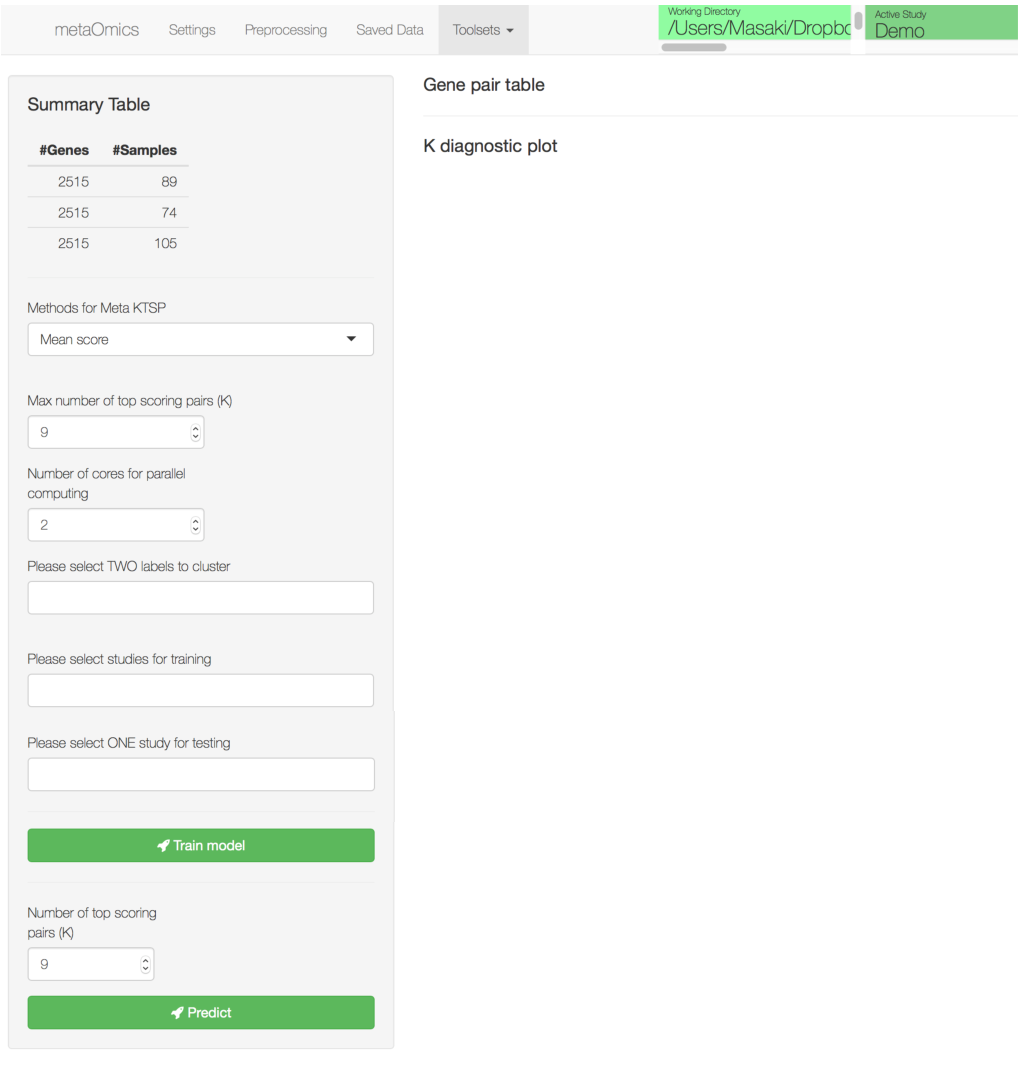
\includegraphics[scale=0.7]{./figure/MetaKTSP/Figure4.pdf}
\caption{Homepage of MetaKTSP}
\label{fig:MetaKTSPmainpage}
\end{center}
\end{figure}

First, we need to decide a method to select K top scoring gene pairs from multiple studies (Figure \ref{fig:MethodSelect}). Second, we need to provide the maximum number of top scoring pairs $K$ (algorithm will search from 1 up to $K$) and the number of cores for parallel computing (Figure \ref{fig:NumK}). Next, we need to select only TWO labels to build the classification model. In other words, if the data exits over two kinds of labels, we need to choose two from them. Our interface will pop up all labels that are available (Figure \ref{fig:TwoLabels}). Then, select the dataset as training data and testing respectively, and click the "Train model" tab to run the MetaKTSP program  (Figure \ref{fig:TrainTest}). It may take a while to run the model.

\begin{figure}[H]
\begin{center}
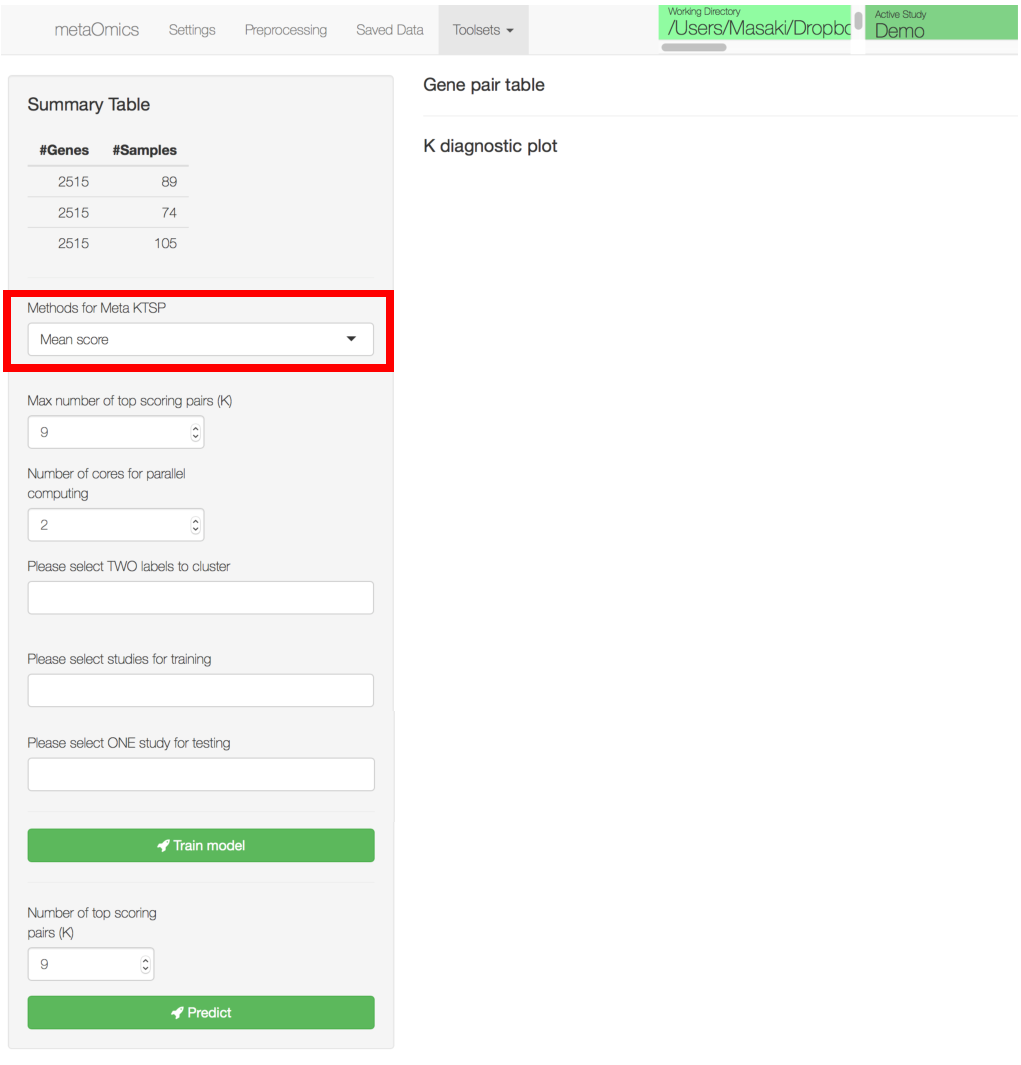
\includegraphics[scale=0.7]{./figure/MetaKTSP/Figure5.pdf}
\caption{Select meta-analysis method.}
\label{fig:MethodSelect}
\end{center}
\end{figure}

\begin{figure}[H]
\begin{center}
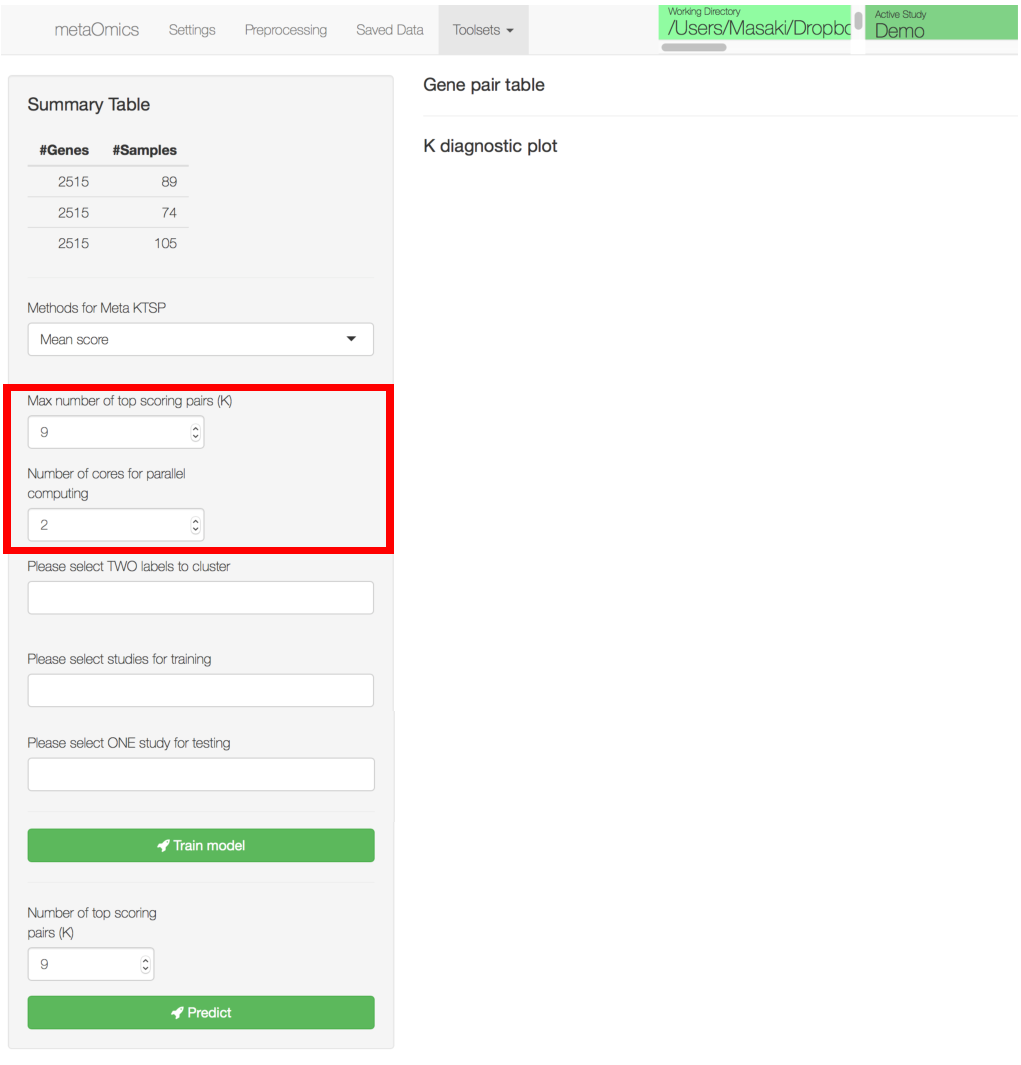
\includegraphics[scale=0.7]{./figure/MetaKTSP/Figure6.pdf}
\caption{Select maximum number of top scoring pairs and number of cores for parallel computing.}
\label{fig:NumK}
\end{center}
\end{figure}

\begin{figure}[H]
\begin{center}
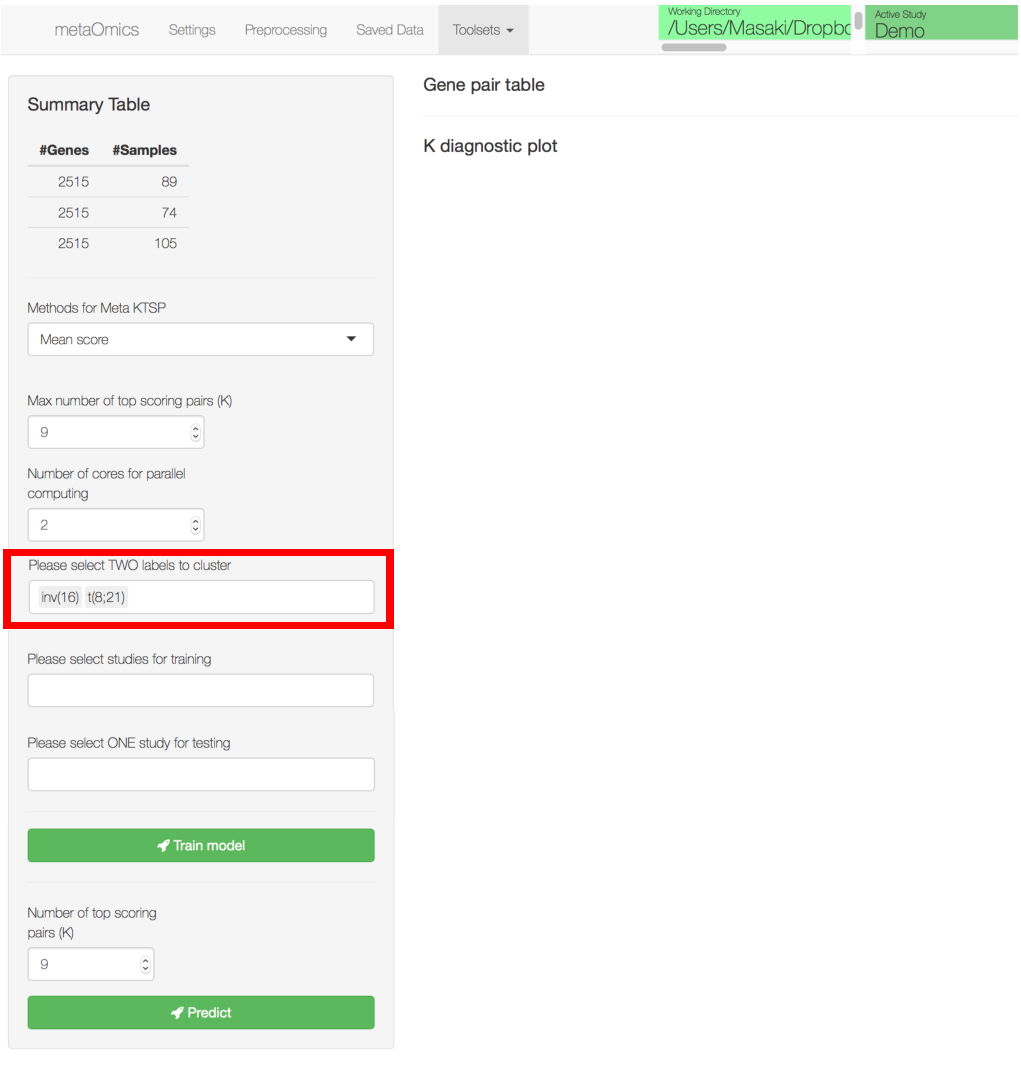
\includegraphics[scale=0.7]{./figure/MetaKTSP/Figure7.pdf}
\caption{Select only two labels to build the classification model.}
\label{fig:TwoLabels}
\end{center}
\end{figure}

\begin{figure}[H]
\begin{center}
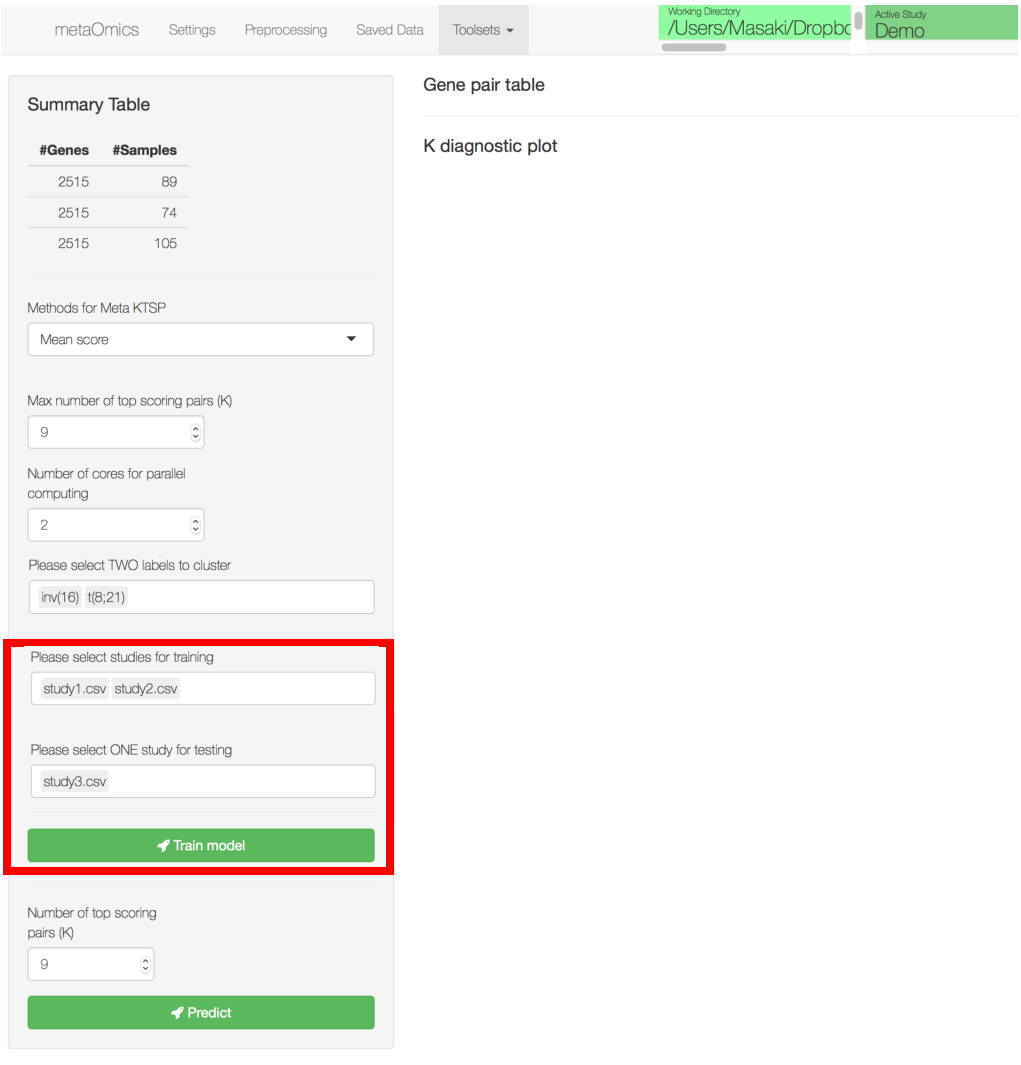
\includegraphics[scale=0.7]{./figure/MetaKTSP/Figure8.pdf}
\caption{Select training dataset and testing dataset and hit the ``Train model" tab to run the MetaKTSP program.}
\label{fig:TrainTest}
\end{center}
\end{figure}

After the model training is finished, on the top right it will show up a ``Gene pair table" which present the top $K$ gene pairs statistics (Figure \ref{fig:PairTable}). As shown in Figure \ref{fig:DiagnosticPlot}, a diagnostic plot is output to assist users decide which $K$ to use in the final prediction model. The suggested value is shown in the plot as green line, which is decided by VO method we introduced in the original paper. Users may also decide $K$ on their own to predict the class label of testing data. After deciding $K$, then hit the tab ``Predict'' (Figure \ref{fig:Predict}). Finally, a confusion matrix is output to show the prediction results (Figure \ref{fig:Confusion}).

%\begin{figure}[H]
%\begin{center}
%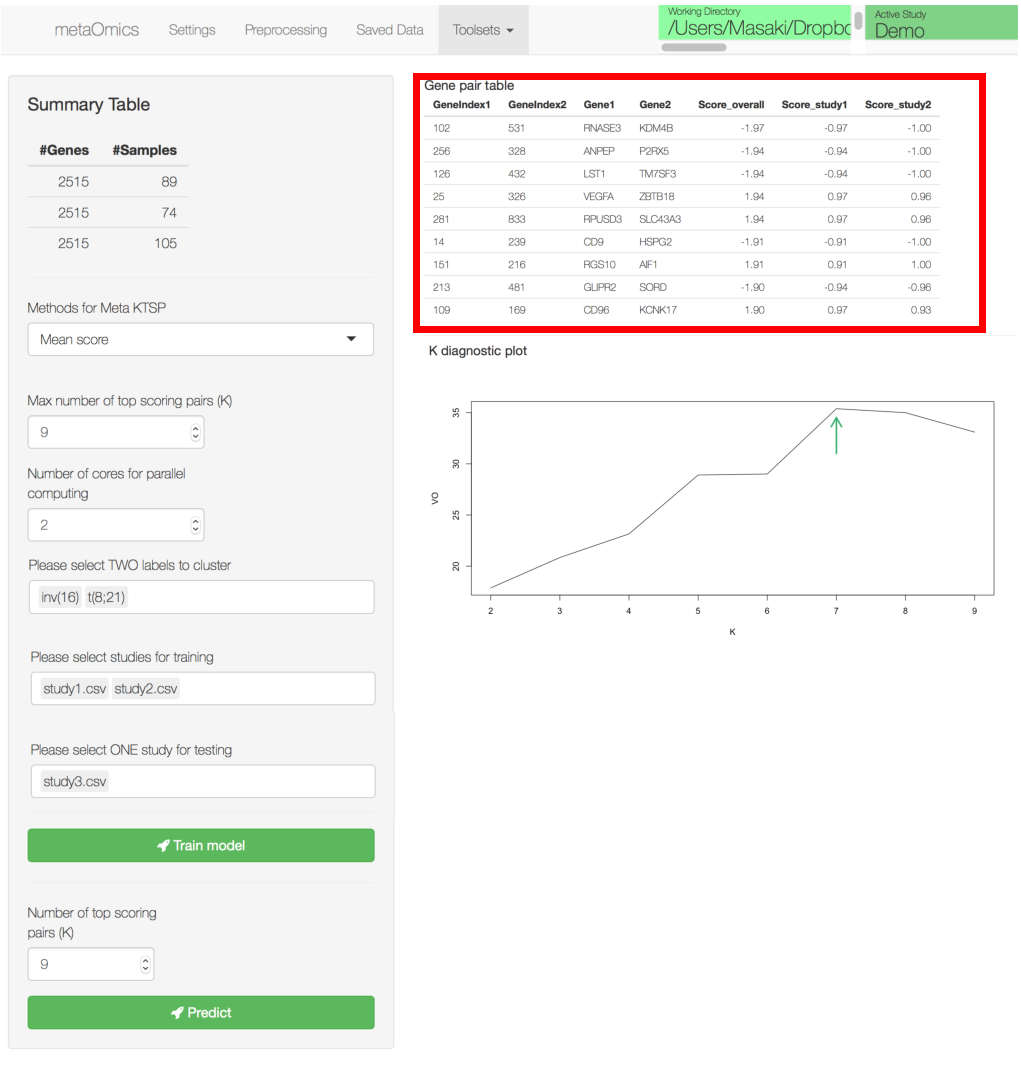
\includegraphics[scale=0.7]{./figure/MetaKTSP/Figure9.pdf}
%\caption{Gene pair table presents the statistics for $K$ top scoring pairs.}
%\label{fig:PairTable}
%\end{center}
%\end{figure}

%\begin{figure}[H]
%\begin{center}
%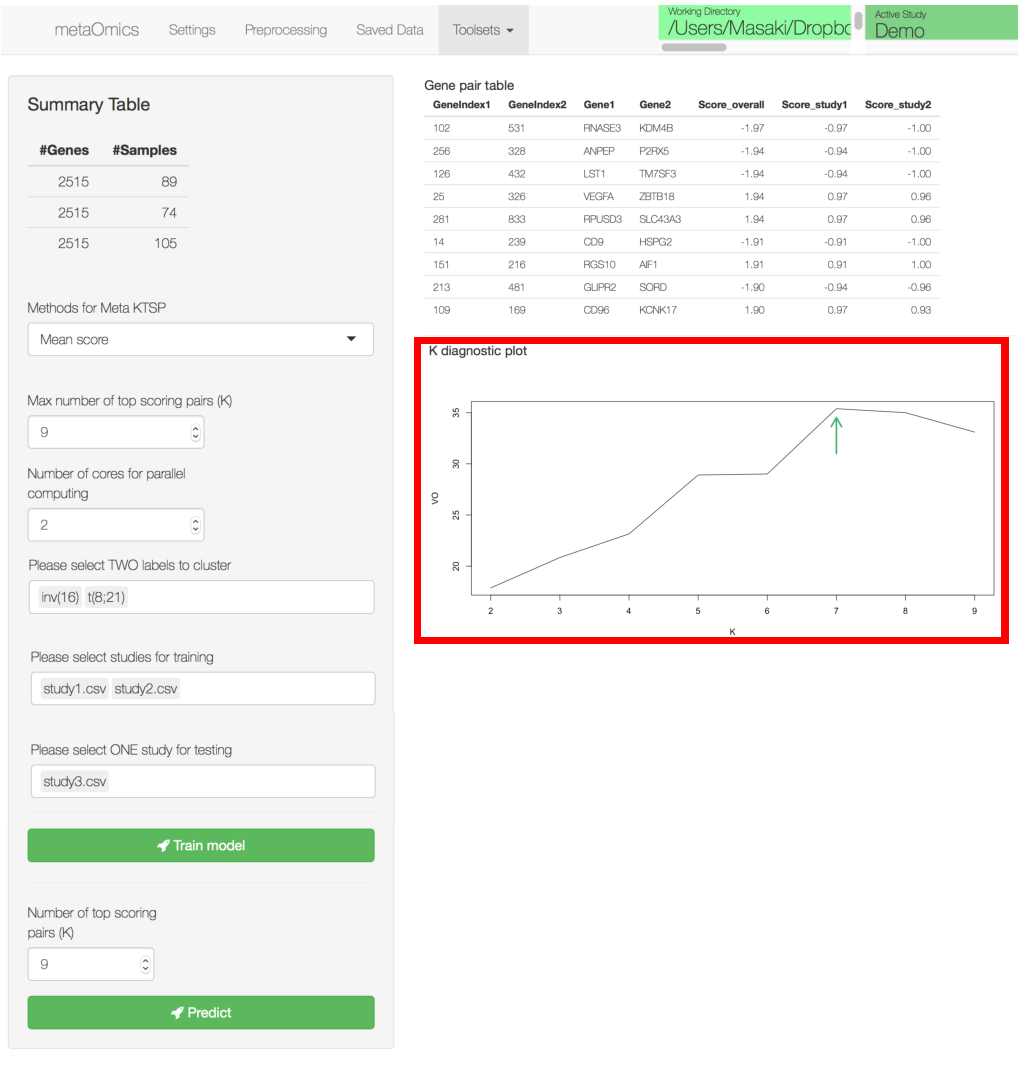
\includegraphics[scale=0.7]{./figure/MetaKTSP/Figure10.pdf}
%\caption{Diagnostic plot for choosing optimal $K$ from training model. It will be used for predicting the class labels for testing dataset.}
%\label{fig:DiagnosticPlot}
%\end{center}
%\end{figure}


%\begin{figure}[H]
%\begin{center}
%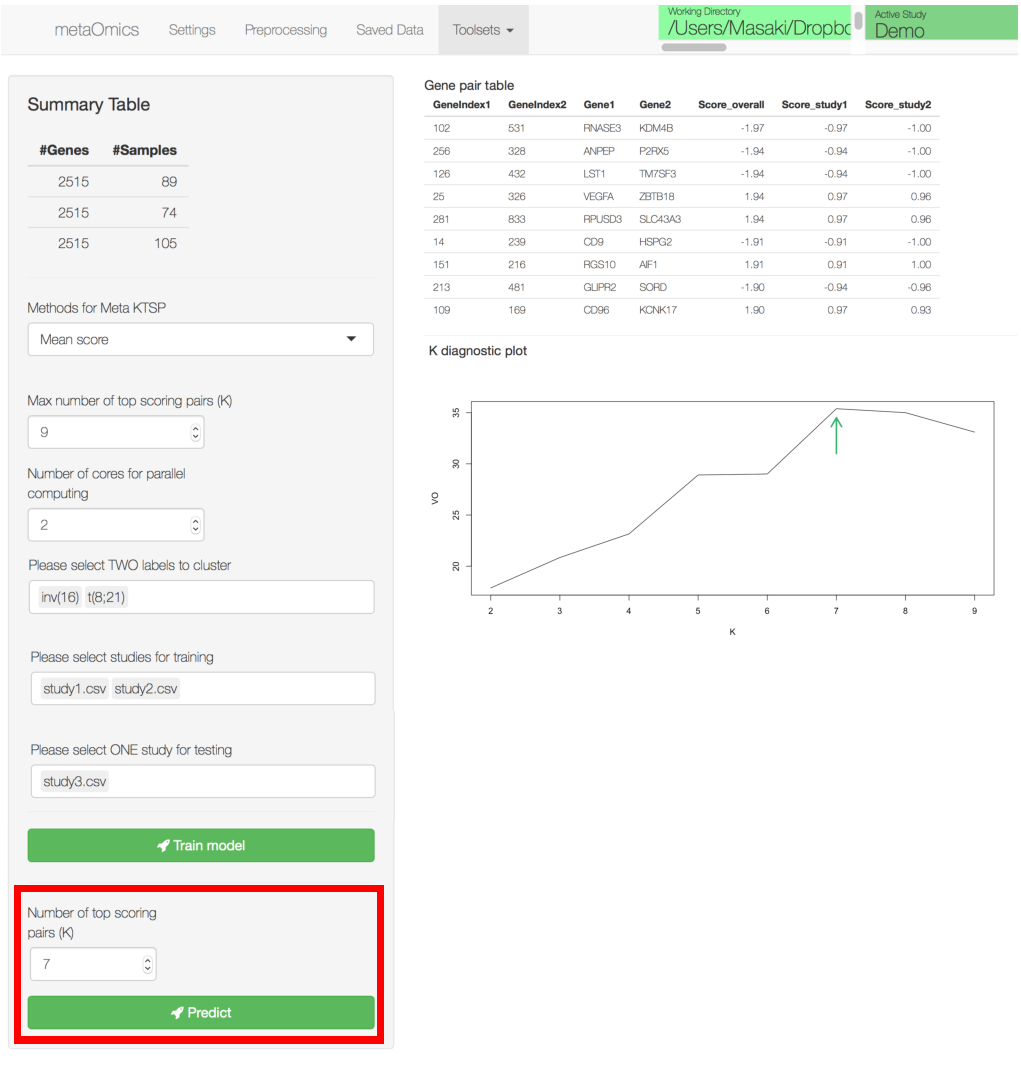
\includegraphics[scale=0.7]{./figure/MetaKTSP/Figure11.pdf}
%\caption{Choose the optimal $K$ for prediction model. Hit tab ``Predict" to perform prediction for testing dataset.}
%\label{fig:Predict}
%\end{center}
%\end{figure}

%\begin{figure}[H]
%\begin{center}
%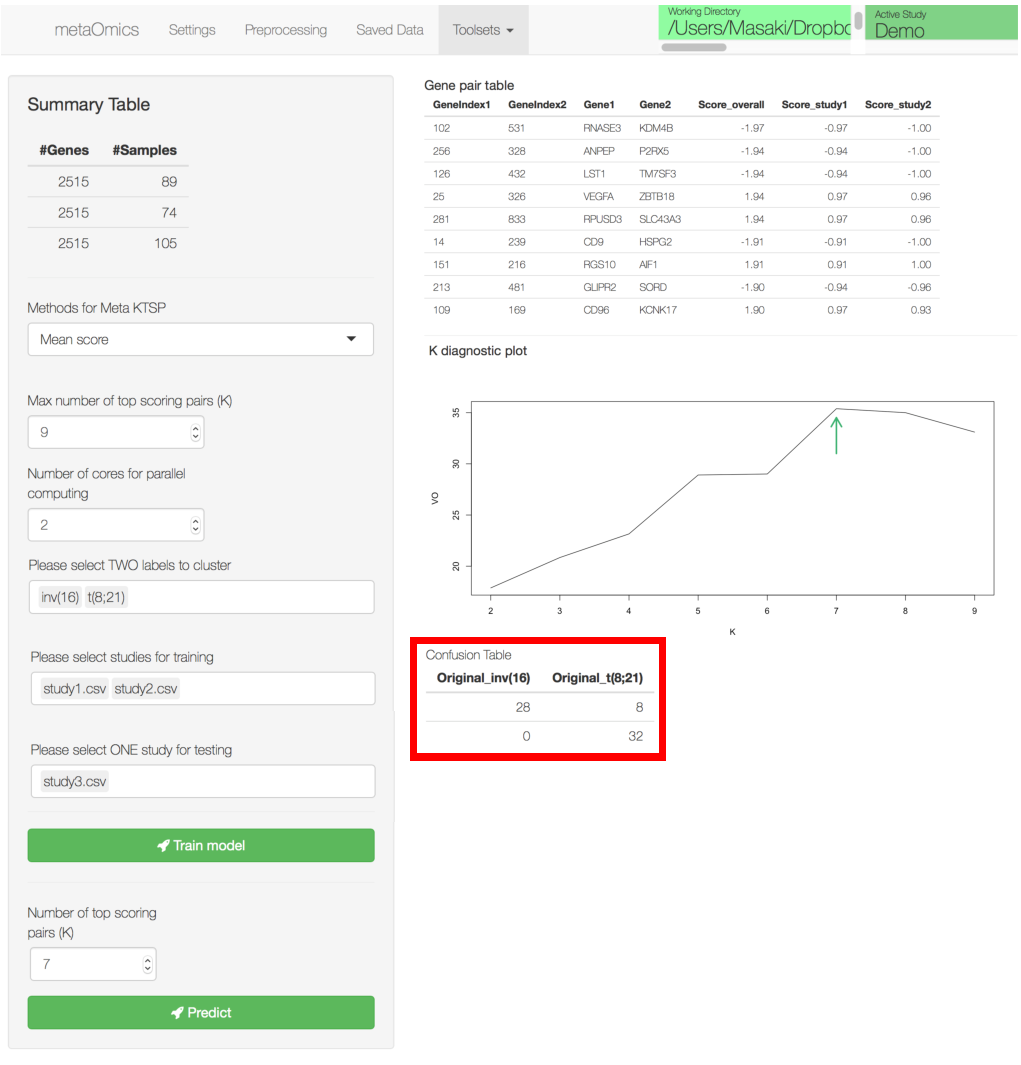
\includegraphics[scale=0.7]{./figure/MetaKTSP/Figure12.pdf}
%\caption{Prediction result based on testing data using 7 top scoring pairs derived from MetaKTSP model. The column of the confusion matrix is the given class label and the row is the prediction result.}
%\label{fig:Confusion}
%\end{center}
%\end{figure}
